\chapter{Software Architecture}
\label{ch:Software_Architecture}

\author{Nico Kratky}
%

After studying lots of literature about real-time systems, a new fundamental software architecture was developed. The main principle of this is to seperate different tasks into seperate processes. This makes use of the fact that the processed data is sent to the client over the internet anyways. Therefore the process that handles data storage also acts as a client. This leads to increased protability, and more important, increased performance. This sofware stack is depicted in figure \vref{fig:gramoc-stack} and its components are further introduced and discussed in the following chapters.

\begin{figure}[!htb]
    \centering
    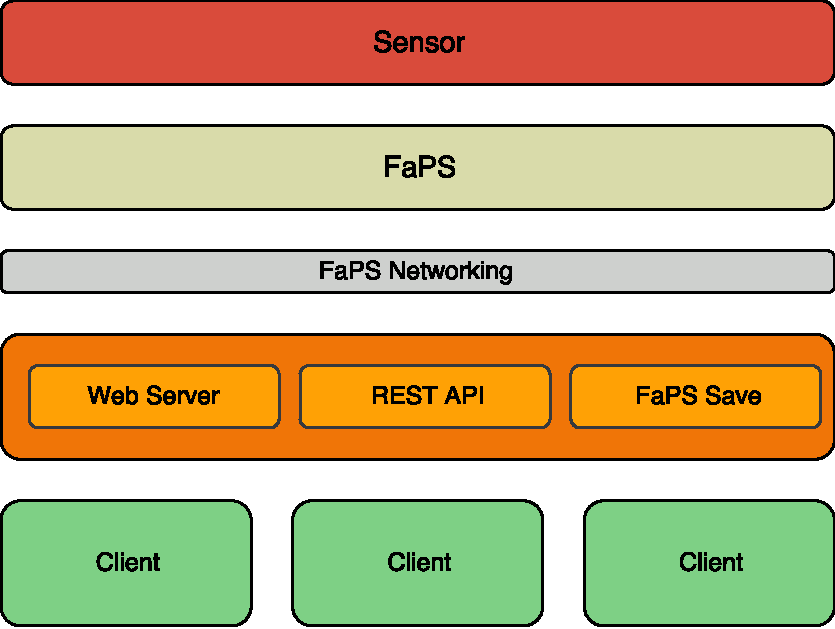
\includegraphics[width=10cm,keepaspectratio]{gramoc-stack}
    \caption{GRAMOC Software Architecture Diagram}
    \label{fig:gramoc-stack}
\end{figure}

